\ifdraft{\tableofcontents
\clearpage
}{}

\section{Introduction} \label{sec:why-this-matters}
Current thinking about AI policy points out considerations related to verification, validity, security and control that can reduce the incidence of surprising behaviour in autonomous systems \cite{research-priorities}, but, so far, less attention has been given to features that would allow these systems to make beneficial use of surprises they encounter in the world. 
%
Nevertheless, related themes have been debated in the philosophy of AI since the dawn of the computing age.  Luigi Menabrea's \cite[p.~689]{menabrea1842sketch} remarks on Babbage's Analytical Engine hinted at an intriguing line of enquiry: ``the interpretation of formulae and of results is beyond its province,'' he wrote, ``unless indeed this very interpretation be itself susceptible of expression by means of the symbols which the machine employs.''  To Ada Lovelace, this suggestion served primarily as evidence of an overwarm reception for an incipient technology.  She did however presciently observe that the complexity of program operations would push the limits of human understanding \cite[p.~710]{lovelace}.
%% \begin{quote}
%% ``\emph{There are frequently several distinct \emph{\textbf{sets of effects}} going on simultaneously; all in a manner independent of each other, and yet to a greater or less degree exercising a mutual influence. To adjust each to every other, and indeed even to perceive and trace them out with perfect correctness and success, entails difficulties whose nature partakes to a certain extent of those involved in every question where \emph{\textbf{conditions}} are very numerous and inter-complicated; such as for instance the estimation of the mutual relations amongst \emph{\textbf{statistical}} ph\ae nomena, and of those involved in many other classes of facts.}'' \cite[p.~710]{lovelace}~{[}emphasis in original{]}
%% \end{quote}

A hundred and twenty five years later, Marvin Minsky described the state of affairs in programming practice.  ``When a program grows in power by an evolution of partially-understood patches and fixes, the programmer begins to lose track of internal details and can no longer predict what will happen'' \cite{minsky1967programming}.
% https://web.media.mit.edu/~minsky/papers/Why%20programming%20is--.html
In the early twenty first century, neural programs are now routinely evolved by computational means, resulting in code and behaviour that no one can claim to fully understand.  The systems that Turing called \emph{learning machines} \cite{turing1950mind} are now part of everyday life.  Although these systems have mastered constrained domains such as Chess and Go, more powerful applications, such as language learning and human-level performance in mathematics \cite{turing1948intelligentreport} are not yet fully developed.     

Like Turing, \citet[p.~2015]{sloman2008well} highlights ``interactions with a complex environment'' as a prerequisite for learning mathematics.  Meaningful interaction often requires more than blind optimisation relative to predefined constraints.  Consider the role of serendipity---the creative interpretation of unexpected discoveries---in the history of science and invention \cite{roberts,van1994anatomy}.

As a route to an improved understanding of autonomous systems, our goal in this paper will be to model serendipity in computationally-feasible terms. In response to a classic objection to the generation of ``pure serendipity'' by computational means \cite{van1994anatomy},  we embrace the concept of \emph{serendipity potential}.
%In Section \ref{sec:literature-review}, 
We draw on a review of prior literature on serendipity and related concepts such as discovery, invention, creativity, and insight.  We assemble a unified framework that summarises the logical structure of serendipitous occurrences.
% In Section \ref{sec:our-model},
This leads us to a process-oriented model of systems with serendipity potential with six constituent phases:
\emph{perception}, \emph{attention}, \emph{interest}, \emph{explanation}, \emph{bridge}, and \emph{valuation}.
We draw on literature in cognitive science and philosophy to define these terms, and examine examples of systems that implement the features of the model.
% In Section \ref{sec:system-analysis},
Although we have not done new implementation work to support our argument, we outline directions for future development.

\section{Background} \label{sec:background}

The concept of serendipity has been adopted for users' benefit by many subfields of computer science, including information retrieval \cite{Toms2000, Andre:2009:XSP:1518701.1519009}, recommender systems \cite{kotkov2016survey} and planning \cite{muscettola1997board, chakraborti2015planning}. For example, the {\sf SerenA} project, developed by \citet{maxwell2012designing}, aimed to support users in forming bridging connections from an unexpected encounter to a previously unanticipated but valuable outcome by drawing on linked data from the web. With {\sf Auralist}, \citet{Zhang2011} present a case-study on serendipity in music recommendation: they increase the unexpectedness of their recommendations by means of a declustering algorithm on item popularity and user profile similarity. \citet{chakraborti2015planning} develop a formal account of planning for serendipity in human-robot interaction: they describe an urban search and rescue scenario where a person must conduct triage in a certain room, and then experiences serendipity when the robot intercepts ``him with a medkit in the hallway so he need not fetch one himself.''

There is a strong bias in the existing technical literature towards ``serendipity as a service'', i.e. to leveraging computer systems to support and catalyse a serendipitous experience in the user. In this article, we propose to switch perspectives from such ``serendipity as a service'' to ``\emph{serendipity in the system},'' where artificial systems catalyse, evaluate and leverage serendipitous occurrences themselves. This perspective shift requires a more nuanced understanding of serendipity.  One strategy would be to consider a reversal of roles in which a person contributes to a system's experience of serendipity in some suitable sense.  However, our central goal is to theorise, and indicate in broad terms how to engineer systems which do not depend on such support by people, but which have the capacity to detect, evaluate and use serendipitous events without user intervention.  Why might such features be useful?  Consider the following point raised by \citet{delamaza1994generate}: ``How disastrous it would be if a discovery system's greatest discovery was `not noticed' because a human did not have the ability to recognise it!''

We fully agree with van Andel that an artificial system cannot be guaranteed to engage in serendipitous findings \cite{van1994anatomy}, just as a person cannot deliberately force serendipity to happen on demand.  However, we still believe that serendipity can happen independently of human intervention within an artificial system, and that the ``\emph{serendipity potential}'' of such a system can be increased by means of a suitable system architecture. 
We will frame our analysis in terms of a current theory in cognitive science known as \emph{predictive processing} (for a recent review, see \cite{newen2018oxford}).   The main hypothesis in this line of work is that such beings are conscious of, and act upon, precisely those data which are found to be unexpected.  Alongside in-built faculties and predispositions, previous experience gives living beings a sense of what to expect. This is said to apply at all levels of mind.  Data that differs from the expected provokes a response: some responses support homeostasis, others drive curiosity, and so on.

Although it is finding new applications in a range of areas, including AI and robotics (see, e.g., \citet{DBLP:journals/corr/McGregorBB15,10.3389/frobt.2018.00021,thornton2017predictive}), the predictive processing framework is also conveniently glossed as ``the latest incarnation of an approach to perception and cognition initiated by Kant and refined by Helmholtz'' \cite{swanson2016predictive}.  Some of these early explorations are relevant to our current concerns.  Kant had contended that ``reason has insight only into what it itself produces according to its own design''---and he disparaged the notion of learning from accidental observations absent ``a previously thought out plan'' \cite[p.~20]{kant1929critique}.  In light of our current considerations it is also natural to wonder what, if anything, can be learned from a previously thought out plan in the absence of accidents.  Kant allowed for new rules to be invented via \emph{reflective judgement}, in a process somewhat akin to unsupervised learning \cite[p.~265]{kant1987critique}.  Reflection is a ``subjective principle governing the purposive use of our cognitive powers'' \cite[p.~266]{kant1987critique}.  Recent work within the predictive processing paradigm posits the (related) subjective sense of `grip' as a driver for curiosity \cite{Kiverstein2017}.

We humans also create ``new cognitive niches, new training regimes and designer environments in which to think'' \cite[p.~265]{pittphilsci10470}.  
Herbert Simon  conceptualised \emph{design} as ``the generation of alternatives and, then, the testing of these alternatives against a whole array of requirements and constraints'' \cite[pp.~128--129]{simon1996sciences}. This process is integral to predictive processing theories. 
The model of serendipity that we will develop in Section \ref{sec:our-model} has structural similarities to the model of design science research developed by \citet{Peffers:2007:DSR:1481765.1481768} (Figure \ref{fig:dsrm}).  However, whereas their Design Science Research Methodology begins with a problem, in our model of serendipity, a problem only emerges after several processing steps.  Our model may be understood as an alternative account of design processes that more fully embraces phenomena.
%% As we indicated above, we do not think it is possible to design serendipity, though it has been recognised that it is possible to design \emph{for} serendipity \cite{newman2002designing}.  In light of the fact that, e.g., ``the basal ganglia is connected to the cortext by at least five separate circuits''
%so that ``online cognitive function cannot be assigned to either the cortical or subcortical component, but instead emerges from their tight coordination''

\begin{figure}
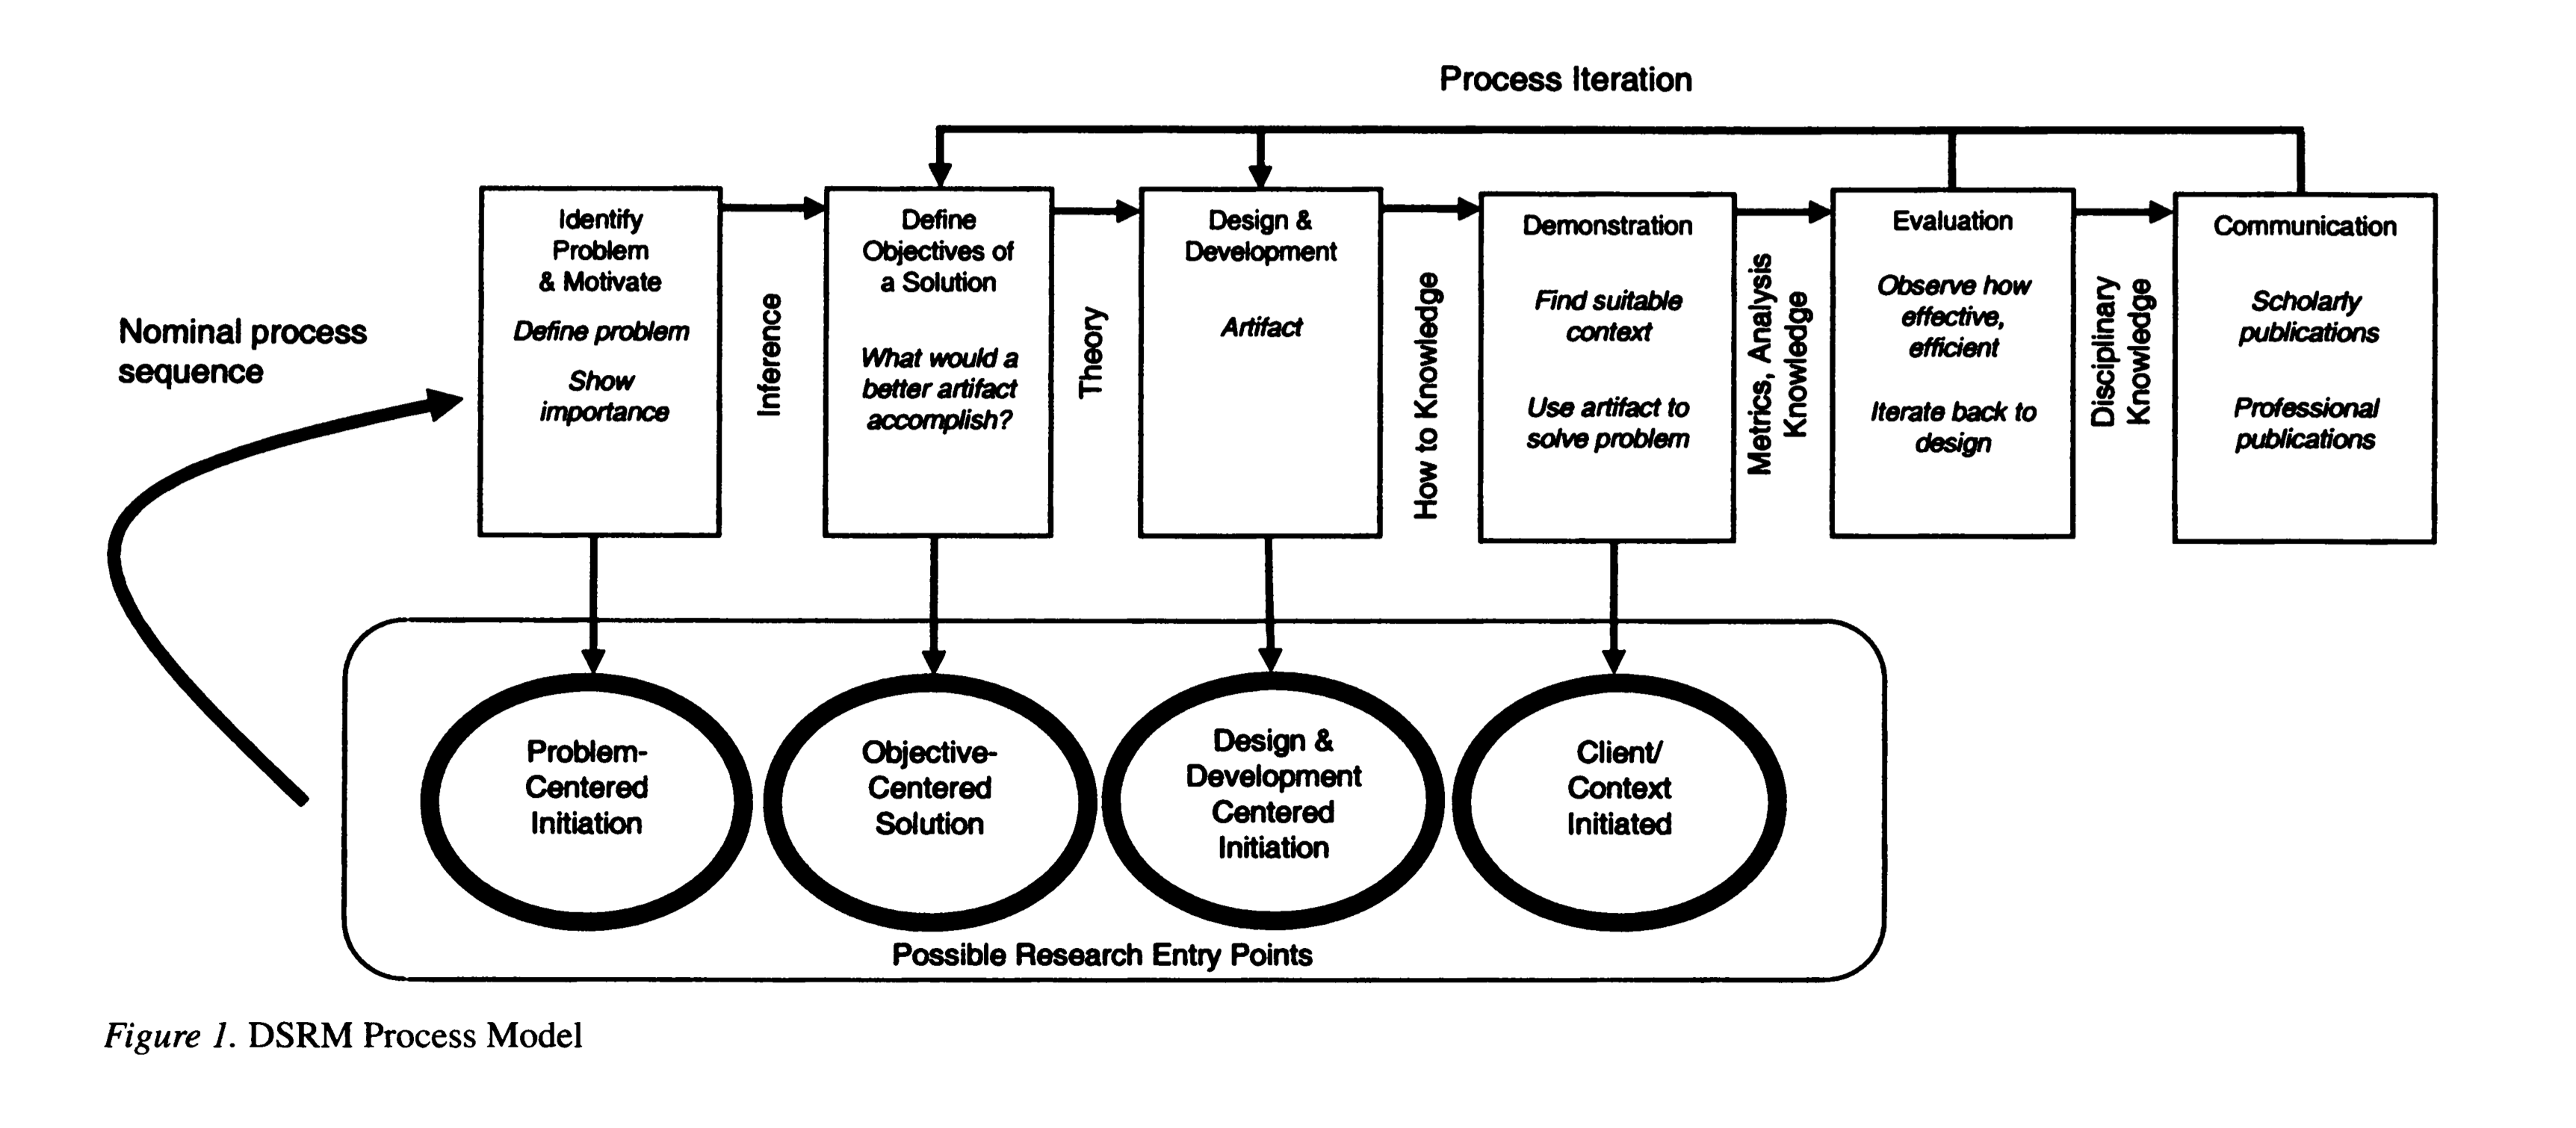
\includegraphics[width=\textwidth,trim={0 3cm 0 0},clip]{pfeffers}
\caption{\citet[p.~54]{Peffers:2007:DSR:1481765.1481768} Design Science Research Methodology (DSRM)\label{fig:dsrm}}
\end{figure}
